\section{McCormick Function}
\label{sec:app:test:mccormick}

  The field of optimization research frequently employs the \emph{McCormick
  function} as an insightful benchmark function. This function owes its name to
  the researcher, Garth P. McCormick, who first employed it in his seminal study
  on factorable nonconvex programs.\footnote{%
    McCormick, Garth P. \enquote{Computability of Global Solutions to Factorable
    Nonconvex Programs: Part I — Convex Underestimating Problems.}
    Mathematical Programming 10, no. 1 (December 1976): 147–75.
    https://doi.org/10.1007/BF01580665.
  }
  The McCormick function is renowned for its oscillatory properties and its
  complex landscape featuring a single global minimum amidst numerous local
  minima.
  This complex landscape can pose a significant challenge to optimization
  algorithms, as they risk being ensnared in the local minima.

  \begin{definition}[McCormick Function]
    The \emph{McCormick Function}, symbolized as \(f: \mathbb{R}^2 \rightarrow 
    \mathbb{R}\), is expressed mathematically as follows:

    \begin{equation}
      \label{eq:app:test:mccormick}
      f(x,\, y) = \sin(x + y) + (x - y)^2 - 1.5x + 2.5y + 1
    \end{equation}

    The McCormick function is typically evaluated within the range \(x,\, y \in
    [-1.5,\,4]\) and \([-3,\,4]\) respectively.
  \end{definition}

  The global minimum of the McCormick function is found at \(f(-0.54719,\,
  -1.54719) \approx -1.9133\). 
  Visualizations of the McCormick function in the form of a contour plot and
  a surface plot are provided in \vref{fig:app:test:mccormick}.

  \begin{figure}[ht!]
    \centering
    \begin{subfigure}[b]{0.45\textwidth}
      \centering
      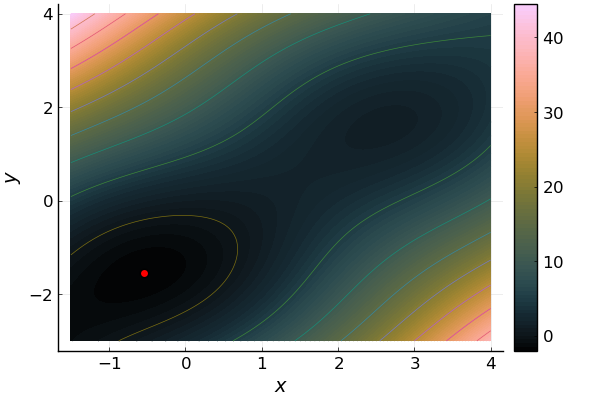
\includegraphics[width=\textwidth]
        {img/test_functions/mccormick_contour.png}
      \caption{
        Contour plot of the McCormick Function.
        The location of the global minimum is designated by a red dot.
      }
    \end{subfigure}
    \hfill
    \begin{subfigure}[b]{0.45\textwidth}
      \centering
      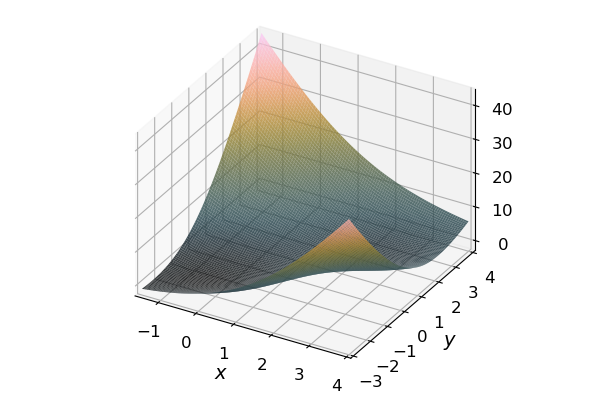
\includegraphics[width=\textwidth]
        {img/test_functions/mccormick_surface.png}
      \caption{Surface plot of the McCormick Function}
    \end{subfigure}
    \caption{Visual representations of the McCormick Function.}
    \label{fig:app:test:mccormick}
  \end{figure}